% (c) 2015 Daniele Zambelli daniele.zambelli@gmail.com

\section{Esercizi}

\subsection{Esercizi dei singoli paragrafi}

\subsubsection*{\numnameref{subsec:iperbole_luogogeometrico}}

\begin{esercizio}
  \label{ese:div.003}
  Considera gli elementi dati nelle iperboli sottostanti e scrivine 
l'equazione.
% \begin{figure}[htbp]
  \centering%
  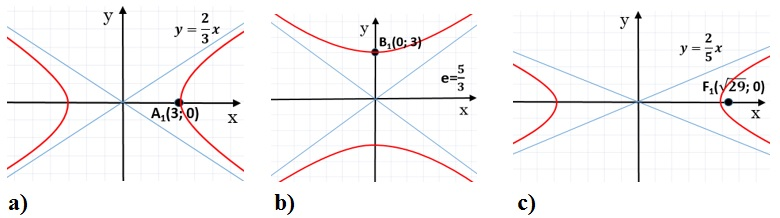
\includegraphics[height=16cm, width=12cm, keepaspectratio] 
{img/graficiip.jpg}%
  %\caption{Generazione di un cono a due falde}%
% \end{figure}
\end{esercizio}

% \vspace{-12pt}
\subsubsection*{\numnameref{subsec:iperbole_caratteristiche}}

\begin{esercizio}
  \label{ese:div.003}
  Determina le misure del semiasse trasverso, del semiasse non 
trasverso e i fuochi delle seguenti iperboli.
  \begin{enumeratea}
  \item $ \dfrac{x^{2}}{25} - \dfrac{y^{2}}{16} =1$
  \hfill $\left[a=5;~ b=4;~ F_{1} \left( \sqrt{41} ;~ 0\right), ~ 
F_{2}  \left(- \sqrt{41} ;~0\right)\right]$
  \item $ \dfrac{x^{2}}{4} - \dfrac{y^{2}}{9} =1$
  \hfill $\left[a=2; ~b=3; ~ F_{1} \left( \sqrt{13} ;~ 0\right), ~ 
F_{2}  \left(- \sqrt{13} ;~ 0\right)\right]$
  \item $ \dfrac{x^{2}}{11} - \dfrac{y^{2}}{5} =1$
  \hfill $\left[a= \sqrt{11} ;~ b= \sqrt{5} ;~  F_{1}  (4; 0), ~ 
F_{2}  (-4; 0)\right]$
  \item $ \dfrac{x^{2}}{16} - \dfrac{y^{2}}{9} =1$
  \hfill   \
    $\left[a=4; b=3; ~ F_{1}  (5 ; 0), ~ F_{2}  (-5 ; 0)\right]$
  \item $ 25x^{2} - 4y^{2} =100$
  \hfill $\left[a=2;~ b=5; ~ F_{1} \left( \sqrt{29} ; ~0\right), ~ 
F_{2}  \left(- \sqrt{29} ;~ 0\right)\right]$
  \item $ x^{2} - y^{2} =49$
  \hfill $\left[a=7;~ b=7; ~ F_{1}  \left(7 \sqrt{2} ; ~0\right),  
F_{2}  \left(-7 \sqrt{2} ;~ 0\right)\right]$
\end{enumeratea}
\end{esercizio}
  
  \begin{esercizio}
    \label{ese:div.003}
    Determina i vertici reali, la semidistanza focale c, 
l'eccentricità e gli asintoti delle seguenti iperboli; infine disegnale.
    \begin{enumeratea}
\item $ \dfrac{x^{2}}{9} - \dfrac{y^{2}}{6} = 1$
\hfill $\left[A(\pm 3; 0);~c= \sqrt{15};~e=\sqrt{\dfrac{5}{3}};~y= 
\sqrt{\dfrac{2}{3}} x,~y=- \sqrt{\dfrac{2}{3}} x\right]$
\item $ \dfrac{x^{2}}{16} - \dfrac{y^{2}}{64} =1$
\hfill $\left[A(\pm4; 0);~c=4 \sqrt{5};~e = \sqrt{5};~y=2x,~y=-2x\right]$
\item $ \dfrac{x^{2}}{18} - \dfrac{y^{2}}{36} = 1$
\hfill $\left[A\left(\pm 3 \sqrt{2};~0\right),~c=3 \sqrt{6};~ 
e=\sqrt{3};~y= \sqrt{2}x,~y= -\sqrt{2} x\right]$
\item 16$ x^{2} -25 y^{2} =400$
\hfill $\left[A(\pm5; 0);~c= \sqrt{41};~e= \dfrac{\sqrt{41}}{5};~ y=  
\dfrac{4}{5}x,~y=-\dfrac{4}{5}x \right]$

\end{enumeratea}
\end{esercizio}

% \vspace{-12pt}
\newpage
\subsubsection*{\numnameref{subsec:iperbole_omografica}}

\begin{esercizio}
\label{ese:div.003}
Disegna le seguenti iperboli equilatere riferite ai propri assi 
determinandone i vertici, i fuochi e la semidistanza focale c.
\begin{multicols}{4}
\begin{enumeratea}
\item $ x^{2} - y^{2} =16$    
\item $ x^{2} - y^{2} =9$ 
\item $ x^{2} - y^{2} =5$         
\item$ x^{2} - y^{2} =-9$
\end{enumeratea}
\end{multicols}
\end{esercizio}

\begin{esercizio}
\label{ese:div.003}
Disegna le seguenti iperboli equilatere riferite ai propri asintoti, 
determinandone i vertici.
\begin{multicols}{4}
\begin{enumeratea}
\item $xy=5$
\item $xy=-4$ 
\item $xy=-7$
\item $xy=16$
\end{enumeratea}
\end{multicols}
\end{esercizio}

\begin{esercizio}
  \label{ese:div.003}
  Dopo aver verificato che le seguenti funzioni rappresentano 
un'iperbole, determinane gli asintoti e il centro di simmetria. Disegna 
infine l'iperbole avendo prima calcolato le sue intersezioni con gli assi.
  \begin{enumeratea}
\item $y= \dfrac{3x+2}{x+3} $
\hfill $\left[asintoti:~ x=-3,~ y=3;~ C(-3;~ 3); ~inters.:~ \left(0;~  
\dfrac{2}{3} \right), \left(- \dfrac{2}{3} ;~ 0\right)\right]$
\item $y= \dfrac{2x+3}{2x+5} $
\hfill $\left[asintoti:~ x=- \dfrac{5}{2} ,~ y=1;~C\left(-\dfrac{5}{2};~ 
1\right);~ inters.:~ \left(0;~  \dfrac{3}{5} \right), \left(- \dfrac{3}{2} 
;~ 0\right)\right]$
\item $y= \dfrac{4-x}{x-5} $
\hfill $\left[asintoti:~ x=5,~ y=-1;~ C(5;~-1);~ inters.:~\left(0;~ 
-\dfrac{4}{5} \right), ~(4;~0)\right]$
\item $y= \dfrac{4x-3}{x-2} $
\hfill $\left[asintoti: ~x=2,~ y=4;~ C(2;~4);~ inters.:~ \left(0; ~ 
\dfrac{3}{2} \right), \left(\dfrac{3}{4};~0\right)\right]$
\item $y= \dfrac{2}{x+3} $
\hfill $\left[asintoti: ~x=-3,~ y=0;~ C(-3;~0);~ inters.:~\left(0;~ 
-\dfrac{2}{3} \right)\right]$
\item $y= \dfrac{3x}{x-1} $
\hfill $\left[asintoti:~ x=1,~ y=0;~ C(1;~0); ~inters.: ~(0;~ 0)\right]$
\end{enumeratea}
\end{esercizio}

% \subsection{Esercizi riepilogativi} TODO
% 
% \begin{esercizio}
% \label{ese:D.19}
% testo esercizio
% \end{esercizio}
% 
% \begin{esercizio}\label{ese:03.1}
% Consegna:
%  \begin{enumeratea}
%   \item  
%  \end{enumeratea}
% \end{esercizio}
